%!TEX root = Constructive Alignment for Introductory Programming.tex

\chapter{Approaches to Constructive Alignment} % (fold)
\label{cha:background}

\graphicspath{{Figures/Background/}}

\cite{DeRaadt:2005} approach to learning  had the strongest correlation to success as compared to other cognitive and demographic measures.

\section{Constructive Alignment} % (fold)
\label{sec:constructive_alignment}

Constructive alignment, as proposed by Biggs~\cite{Biggs:1996c}, is an amalgamation of constructive learning theory and aligned instruction design. It aims to elicit deep learning approaches from all students. Biggs' model is student focused, with clear and intentional alignment of assessment, teaching and learning activities, and unit objectives. The focus on the central role of the learner in building meaning is derived from constructivist learning theories, whilst the alignment of assessment, teaching, and learning activities, has its foundation in instructional design literature. 

\fref{fig:constructive_alignment} illustrates the constructive alignment model presented in~\cite{Houghton:2004}, which consists of the following blocks:

\begin{itemize}
	\item \emph{Intended learning outcomes} clearly define required learning in terms of ``performances of understanding''.
	\item \emph{Performance objectives} emerge from the desired outcomes, and can be ranked to become the assessment criteria.
	\item \emph{Teaching and learning activities} are designed to place students in situations likely to elicit the required learning.
	\item Students provide \emph{evidence of their learning}, that is assessed against the criteria to determine grade outcomes.
\end{itemize}

% \begin{figure}[t!]
% 	\centering
% 	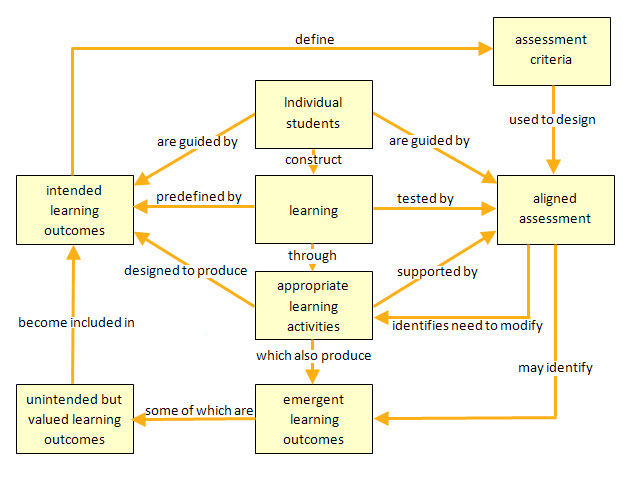
\includegraphics[width=\columnwidth]{Houghton_constructive_alignment_1}
% 	\caption{Constructive alignment model presented by Houghton in~\cite{Houghton:2004}}
% 	\label{fig:constructive_alignment}
% \end{figure}

\subsection{Constructivism} % (fold)
\label{sub:constructivism}

In designing teaching and learning contexts, educators use some form of theory of teaching and learning to guide their decision making.

theory of teaching and learning

espoused theory \cite{Argyris:1976}

\emph{objectivist}

\emph{constructivism} and \emph{phenomenography}


\cite{Duffy:1996} 




\cite{Montessori:1946}

Constructivism is a theory of knowledge that focuses on the active role of the learner in constructing their own understanding. Dating back to \citet{Piaget:1950} constructivism exists in several forms: cognitive, individual, postmodern, radical and social constructivism \cite{Phillips:1995,Steffe:1995}. Each of these forms of constructivism has various implications for teaching and learning.









In his original paper on constructive alignment \citet{Biggs:1996c} adopted constructivism as a framework to help guide decision making in all facets of teaching and learning. Constructivism was chosen over phenomenography 

practical concerns


For this work we are interested in adapting \emph{constructive learning theories}

 taking practical aspects from constructivism in general and focusing on what the student does, as suggested by .


In proposing constructive alignment, 

Disconnect between theory in use and espoused theory: \cite{Phillips:2005}


Engage with and expand experience \cite{Dewey:1960} exploration, thinking and reflection

% subsection constructivism (end)

\subsection{Aligned Curriculum} % (fold)
\label{sub:aligned_curriculum}

% subsection aligned_curriculum (end)


% section constructive_alignment (end)

\clearpage
\section{Reported Applications of Constructive Alignment} % (fold)
\label{sec:reported_applications_of_constructive_alignment}

In this section we outline a literature review that examined the applications of constructive alignment in Higher Education. This review aimed to help identify how constructive alignment can be applied to introductory programming, and any gaps in the current research literature. 

\subsection{Review Method} % (fold)
\label{sub:review_method}

\citet{Petticrew:2008} define a structure literature review as a process of systematically analysing all available studies in order to answer specific research questions.This work followed the structured literature review process of \citet{Kitchenham:2004}, and aimed to identify all available studies on how Constructive Alignment has been applied in Higher Education.

\fref{fig:struct_review_proc} shows the three phases in the structured literature review carried out in this work. The first phase identified appropriate search and filter criteria to be used in locating associated literature. In Phase 2, the search criteria is used to identify potentially relevant articles from the indicated sources. The articles identified are then filtered using the filter criteria to identify the relevant articles to pass on to Phase 3, where relevant data is collected from the articles are the analysis performed.

\begin{figure}[tbph]
	\centering
	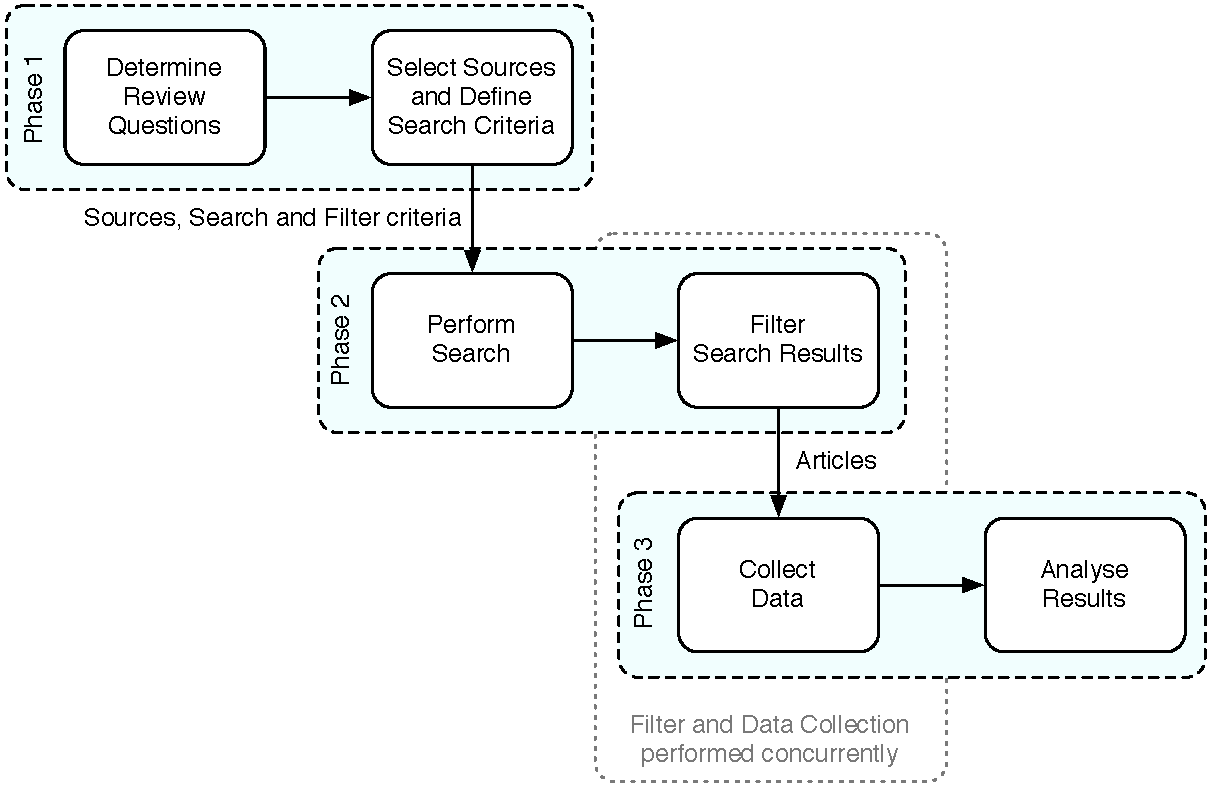
\includegraphics[width=\textwidth]{SystematicReview}
	\caption{Processes in the Structured Literature Review process carried out in this work}
	\label{fig:struct_review_proc}
\end{figure}



\subsubsection{Phase 1: Search and Filter Criteria} % (fold)
\label{sub:review_questions}

This review focused on the application of constructive alignment, and the effectiveness of the teaching and learning environment created. \citet{Petticrew:2008} suggest that the formulation of research questions for a systematic review should consider five aspects: Population, Intervention, Comparison, Outcome and Context (PICOC). Addressing these five aspects enable effective search and filter criteria, that will then be used to identify related work for the review to analyse.

\tref{tbl:picoc} lists the five PICOC aspects related to this review. The Population consists of the specific target group that the study will examine. In this study, the population included students and academics in the context of Higher Education. This work aimed to review interventions where academics had applied the principles of Constructive Alignment, and any comparisons they had with their existing approaches to teaching and learning. In terms of outcomes, we were interested in examining any positive or negative impacts these changes had on either the staff or the students.

\begin{table}[t]
	\centering
	\caption{Focus for database search using PICOC}
	\label{tbl:picoc}

    \begin{tabular}{|l|p{9cm}|}
    \hline
    \textbf{Population} & Students and Academics in Higher Education\\ \hline
    \textbf{Intervention} & Applications of Constructive Alignment in the design of teaching and learning activities and assessment. \\ \hline
    \textbf{Comparison} & Existing approaches \\ \hline
    \textbf{Outcomes} & Positive and negative impacts on student learning, as well as impacts on teaching staff. \\ \hline
    \textbf{Context} & Application of Constructive Alignment to the design and delivery of teaching and learning material in a Higher Education setting. \\ \hline
    \end{tabular}
\end{table}


This structured literature review aimed to answer the following questions:

\begin{enumerate}[noitemsep,nolistsep]
	\item What evidence is there of studies on the application of constructive alignment to teaching and learning in higher education?
	\item How has the effectiveness of constructive alignment been measured in these studies, and how effective has constructive alignment been in the higher education setting?
	\item What teaching and learning activities are used in conjuncture with constructive alignment?
	\item What forms of assessment have been used with constructive alignment?
	\item In what ways have applications of constructive alignment addressed the two main elements of constructive alignment: constructivism and aligned curriculum?
\end{enumerate}

\citet{Petticrew:2008} described the need for the search criteria to result in high number of relevant articles, while excluding irrelevant ones. These are referred to as the search criteria sensitivity and specificity. A search with high sensitivity returns a high number of relevant articles, one with high specificity a low proportion of irrelevant articles. While an ideal search criteria would be both highly sensitive and highly specific, there generally tends to be a trade-off between the two. 

\citet{Kitchenham:2004} provides a number of recommendations on how to define appropriate search criteria, including the use of Boolean AND and OR conditions as well as searching for synonyms. Using this approach results in a search with higher specificity, and can result in a low number of articles being identified, see \citet{Salleh:2011} for example. Therefore, for this work it was decided to start with a highly \emph{sensitive} search criteria, and search for articles that match the term ``Constructive Alignment''. If this resulted in a unacceptably large number of results then more specific criteria could be added.

Given the highly sensitive search criteria, a high number of irrelevant articles was anticipated. To address this, Phase 1 also defined a number of filter conditions. These conditions aimed to clearly define why papers would be excluded from the analysis in Phase 3. The following list shows the criteria used.

\begin{itemize}[noitemsep,nolistsep]
	\item The full text of the paper must be available to the researchers, and must be published in English.
	\item The paper must appear in a peer refereed conference, journal or workshop.
	\item Constructive Alignment must be mentioned, and discussed.
	\item Results must relate to the use of Constructive Alignment in a teaching and learning context.
\end{itemize}

% subsection research_questions (end)

\subsubsection{Phase 2: Identification of Relevant Literature} % (fold)
\label{ssub:identification_of_relevant_literature}

In Phase 2, the search and filter criteria from Phase 1 were used to carry out the search on the selected online databases. The resulting articles were collected in an academic reference management system, that allowed articles to be categorised using a status and a number of tags. Categories were created to indicate why a paper had been excluded, and to mark each paper's progress through the data collection. 

Database searches were performed within the reference management system, which provided facilities to automate the collection of the citation data and the associated full text. Where the full text was not available from the database, a general search was performed using a number of search engines in order to ensure the full text was included for as many articles as possible. This import process also identified any references that were already included in the system, thereby avoiding the creation of duplicates in the resulting library.

The use of the categorisation tools in the academic reference management system allowed the Filter stage of Phase 2 and the Data Collection stage of Phase 3 to run concurrently. Once imported, each article was placed in a \textbf{To Be Categorised} status, thereby providing a backlog of the articles that were to be examined. Each of these articles was then examined using the filter criteria, and moved to a separate status as the filter process progressed. The stages of this process are shown in \fref{fig:filter_proc}.

\begin{figure}[tbph]
	\centering
	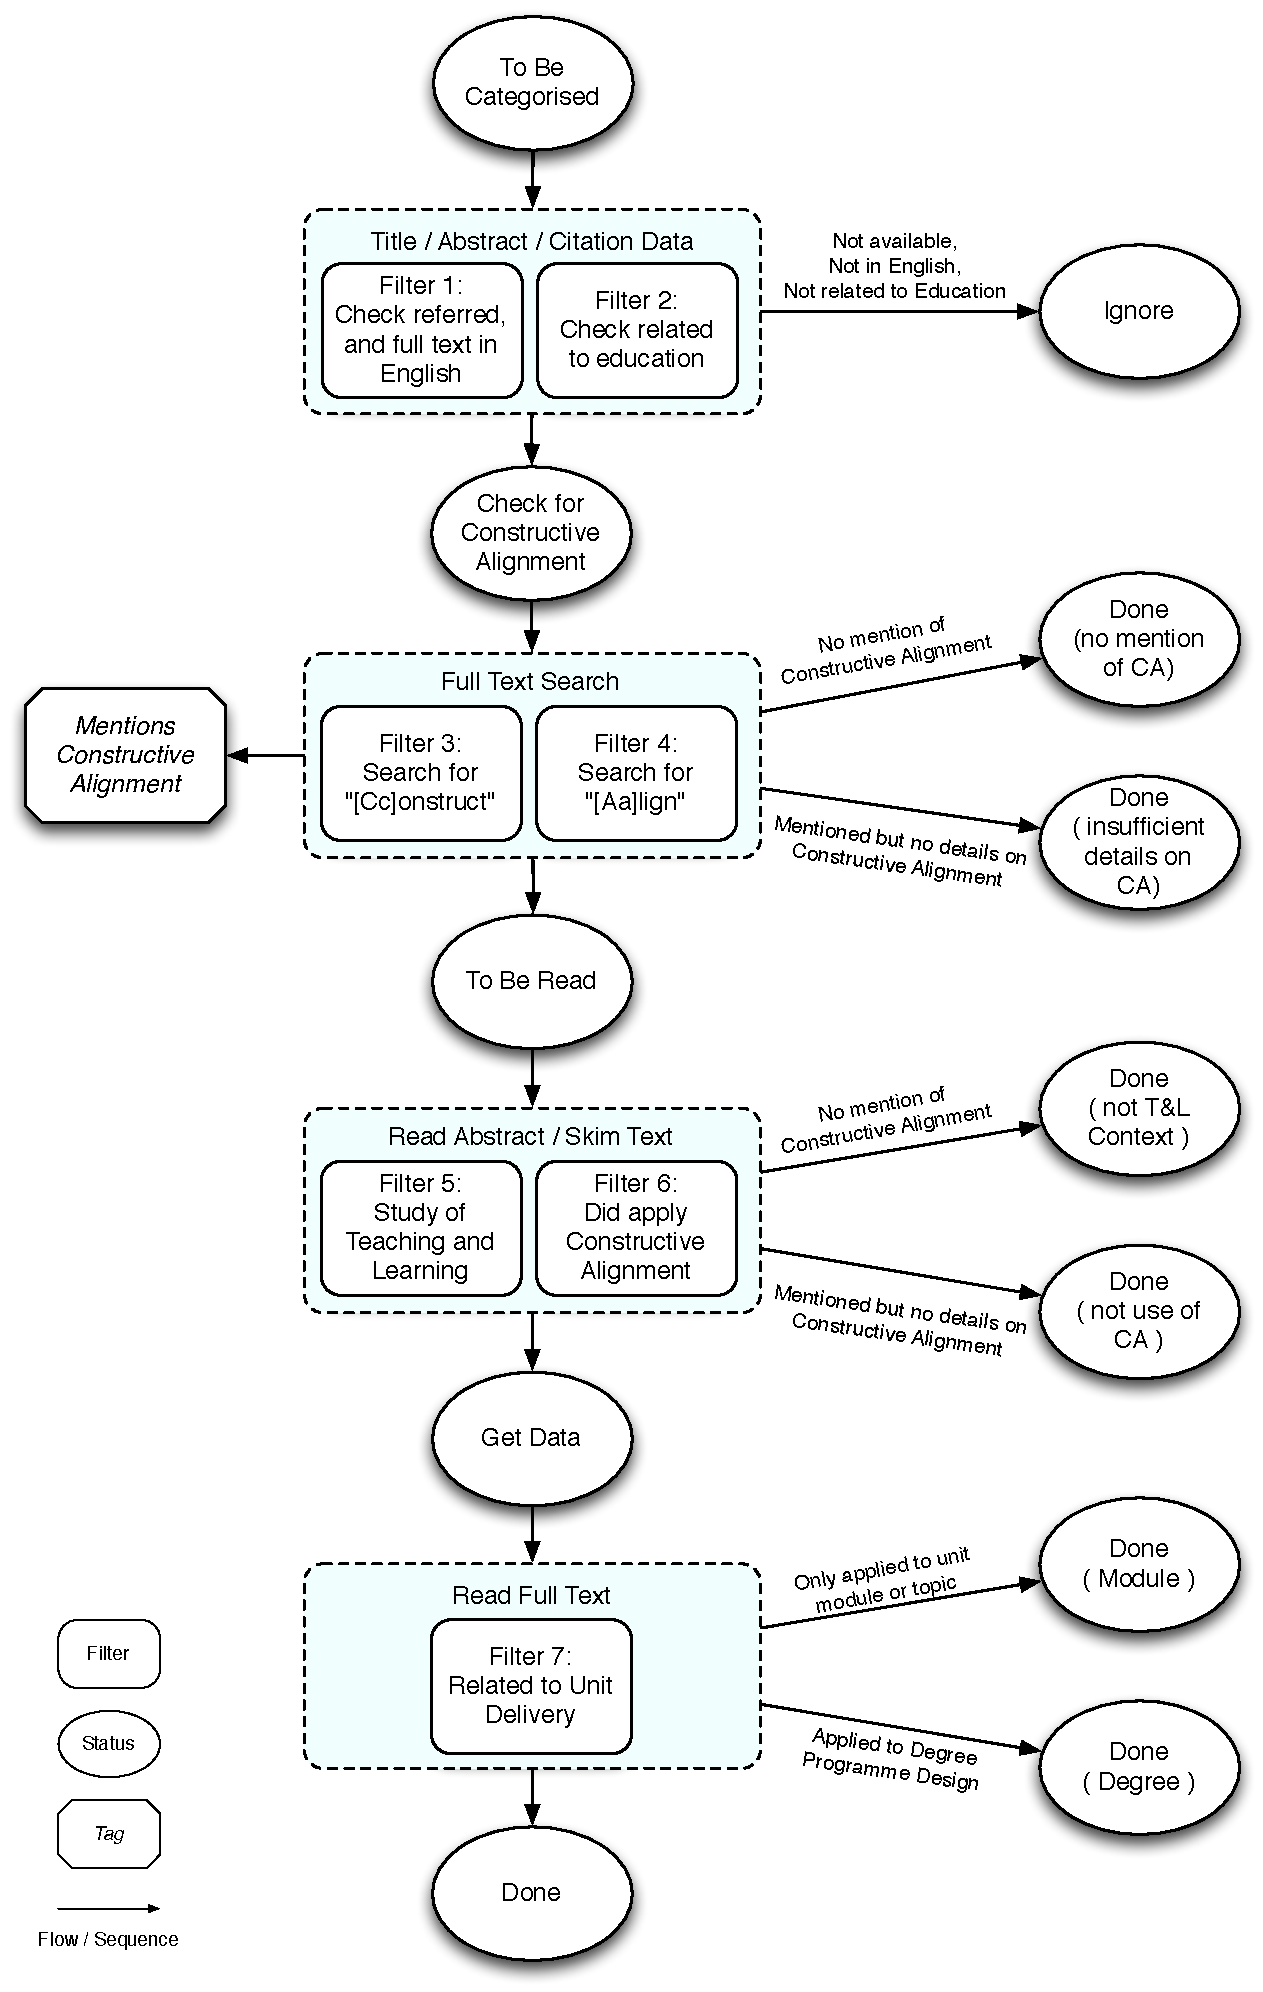
\includegraphics[width=\textwidth]{FilterProcess}
	\caption{Filter process applied to papers}
	\label{fig:filter_proc}
\end{figure}

In the first stage of the filter process the availability of full text, the language it was written in, and its refereed status was checked. If these were not met the paper was allocated to the \textbf{Ignore} status, and did not proceed to the next stage of the filter. 

At the next stage a full text search was conducted on each paper. This search looked for the presence of any text related to constructivism or alignment through the search strings ``construct'' and ``align''. The associated text was then read, and the paper was allocated to \textbf{Done (no mention of Constructive Alignment)} when there was no presence of either words, to \textbf{Done (insufficient details on Constructive Alignment)} when it was mentioned briefly with no details or in depth discussion, and to \textbf{To Be Read} in all other cases. All papers that had mentioned Constructive Alignment were tagged at this stage.

Stage 3 involved reading the abstracts, and all sections related to Constructive Alignment from the papers in the To Be Read status. A new status was allocated to each paper: \textbf{Done (not a Teaching and Learning Context)} if they were a discussion of education theory rather than a study of a teaching and learning context, \textbf{Done (not an application of Constructive Alignment)} if they mentioned Constructive Alignment but had not adopted it for the reported work, and \textbf{Get Data} in all other cases.

The final stage involved reading the full text of the papers in the Get Data status, and classifying them based on what Constructive Alignment had been applied to. Data was collected from all of the papers at this stage, but only those related to the delivery of a unit were forwarded to the analysis phase.

% subsubsection identification_of_relevant_literature (end)

\subsubsection{Phase 3: Data Collection and Analysis} % (fold)
\label{ssub:data_collection_and_analysis}

Data collection was performed by reading the indicated papers and looking for the details in the following list. Findings were recorded in a spreadsheet for further analysis, with relevant quotes from the text being stored alongside the summarised information.

\begin{itemize}[noitemsep,nolistsep]
	\item Level of Unit: Undergraduate, Postgraduate and/or year level.
	\item The Intended Learning Outcomes and associated levels from the SOLO taxonomy.
	\item Teaching and Learning activities used.
	\item Approach to assessment.
	\item Reported effects of constructive alignment.
\end{itemize}

In keeping with the holistic nature of the assessment approaches suggested in \cite{Biggs:1997}, the quality measure for each paper was generated by response to the following question using a five point Likert scale \cite{Likert:1932}: 5 being strongly agree, 4 agree, 3 neutral, 2 disagree, and 1 strongly disagree.

\begin{quote}
``The paper clearly communicates how constructive alignment was applied to the unit, and the results obtained. ''	
\end{quote}

Once all of the data had been collected the details were summarised in the spreadsheet, and analysed to answer the review questions.

% subsubsection data_collection_and_analysis (end)


% subsection review_method (end)
\clearpage
\subsection{Results} % (fold)
\label{sub:review_results}

The search involved the use of seventeen online databases, all of which were searched for the term ``Constructive Alignment''. \tref{tbl:review_source} lists the number of results from each of the selected databases. Google Scholar and CiteSeer resulted in an overly large number of articles for the selected search term. In both cases the results appears to have a large number of irrelevant matches, and so the search terms were updated. The search in Google Scholar was updated to use the term ``intitle:``Constructive Alignment'''', while CiteSeer was limited to searching abstracts for the associated text.

\begin{savenotes}
\begin{table}[ht]
	\centering
	\caption{Data sources and the number of articles located for the search term ``Constructive Alignment''.}
	\label{tbl:review_source}
	\footnotesize
    \begin{tabular}{l|l|c}
    \textbf{Source} & \textbf{URL} & \textbf{Count} \\ \hline
    A+ Education & \url{http://search.informit.com.au/search} & 44 \\
    Academic Search Complete & \scriptsize \url{http://ebscohost.com/academic/academic-search-complete} & 32 \\
    ACM Digital Library & \url{http://dl.acm.org} & 21 \\
    CiteSeer\footnote{With CiteSeer the search was performed on article abstracts containing the text ``Constructive Alignment''.}  & \url{http://citeseerx.ist.psu.edu} & 20 \\
    EdResearch Online & \url{http://opac.acer.edu.au:8080/edresearch} & 6 \\
    Educational Research Abstracts & \url{http://www.tandfonline.com} & 26 \\
    Education Research Complete & \scriptsize \url{http://ebscohost.com/academic/education-research-complete} & 48 \\
    eJournals & \url{http://ejournals.ebsco.com} & 42 \\
    ERIC & \url{http://www.eric.ed.gov} & 31 \\
    Google Scholar\footnote{The search in Google scholar returned more than three thousand results, this was then limited to articles that included ``Constructive Alignment'' in their title.} & \url{http://scholar.google.com} & 104 \\
    IEEE Xplore & \url{http://ieeexplore.ieee.org} & 16 \\
    Libra & \url{http://academic.research.microsoft.com} & 87\\
	PsycINFO & \url{http://ebscohost.com/academic/psycinfo} & 16 \\
	Scopus & \url{http://www.scopus.com/} & 79 \\
	Springer Link & \url{http://link.springer.com} & 125 \\
	VOCED & \url{http://www.voced.edu.au} & 28 \\
	Web of Knowledge & \url{http://wokinfo.com} & 52 \\ \hline
	Total Unique & & 335 \\
    \end{tabular}
\end{table}
\end{savenotes}

When all of the papers were collected in the reference management system a total of 335 unique articles were identified. These articles were then filtered using the process indicated in \sref{ssub:identification_of_relevant_literature}, resulting in 38 papers being included in the final analysis. \tref{tbl:exclude_reason} and \fref{fig:filter_results} show the number of papers excluded by each filter.

\begin{table}[p]
	\centering
	\caption{Counts of number of papers excluded by the indicated filters}
	\label{tbl:exclude_reason}
	\footnotesize
    \begin{tabular}{ll}
    \textbf{Reason} & \textbf{Count} \\ \hline
    No access to full text, or not peer refereed & 77 \\
    No Mention of Constructive Alignment & 33 \\
    No depth of discussion on Constructive Alignment & 96 \\
    Not a study of a Teaching \& Learning Context & 43 \\
    Not an application of Constructive Alignment & 23 \\
    Earlier versions of papers, removed as a duplicate & 10 \\
    Applied Constructive Alignment to Module within Unit & 8 \\
    Applied Constructive Alignment to Degree Programme Design & 7 \\ \hline
    Applied Constructive Alignment to Unit Delivery & 38 \\
    \end{tabular}
\end{table}

\begin{figure}[p]
	\centering
	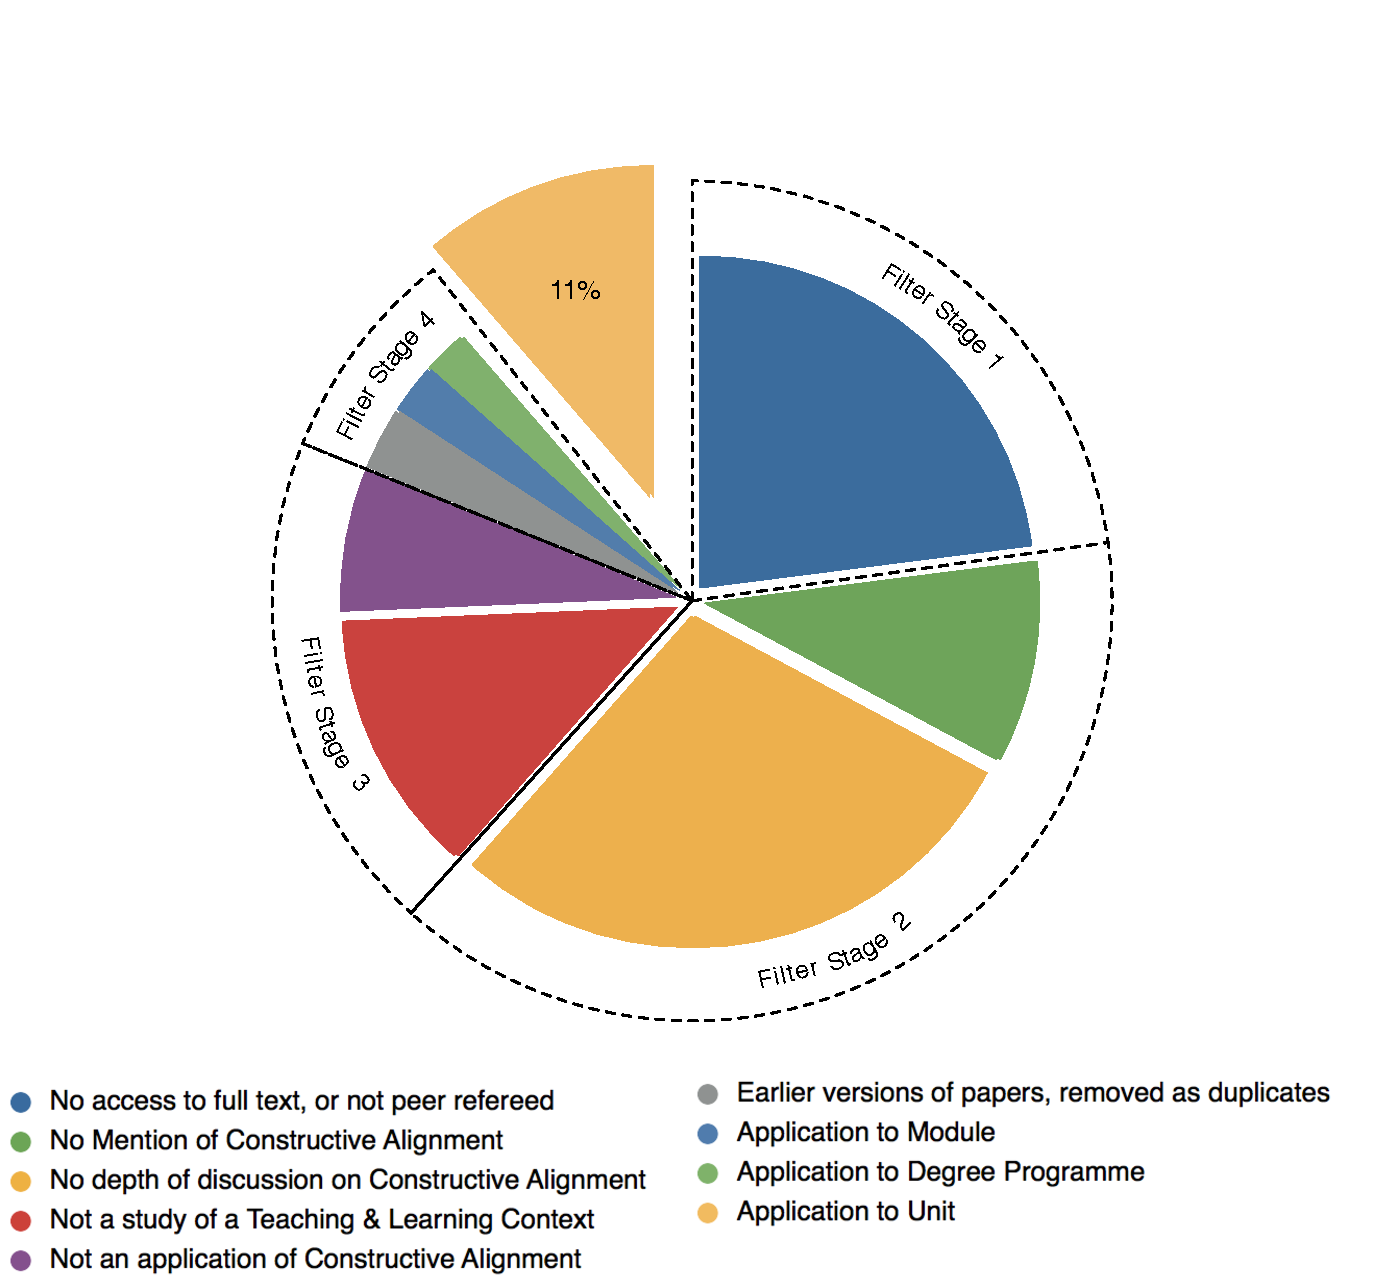
\includegraphics[width=\textwidth]{FilterResults}
	\caption{Pie chart showing the proportion of papers in each status based on the stage excluded by the filters}
	\label{fig:filter_results}
\end{figure}

\clearpage
\subsection{Teaching and Learning Activities} % (fold)
\label{sub:teaching_and_learning_activities}

Units in the analysed papers were primarily delivered face to face (82\%), with only four being delivered online (11\%), and the remaining units having a combination of online and face to face delivery. These results are included in \tref{tbl:delivery}. 

\begin{table}[htbp]
	\centering
	\caption{Method of Unit delivery}
	\label{tbl:delivery}
	\footnotesize
    \begin{tabular}{l|c}
    \textbf{Delivery} & \textbf{Count} \\ \hline
    Face to Face & 31 \\
    Face to Face \& Online & 4 \\
    Online & 3 \\
    \end{tabular}
\end{table}

In the papers that included face-to-face delivery, the data collection examined the types of classes used. The results of this are included in \tref{tbl:class_types}, which lists the number, and percentage, of the papers that reported using lectures, various kinds of tutorials, and other teaching and learning activities. \tref{tbl:class_types} also records the number of papers in which there was no clear communicate of what kind of teaching and learning activities were used.

The four papers in the \emph{Other} category included:
\begin{itemize}[noitemsep,nolistsep]
	\item \citet{Szili:2011} reported using a four day field camp to visit the scene of a serious environmental crisis, as part of a unit related to environmental management.
	\item \citet{donnisonre} who included twenty hours of community service, as part of a unit in the first year of an degree in Education.
	\item Eight weeks of clinical practice \citet{Tang:1999}, as part of a nursing degree.
	\item \citet{Shoufan:2010:CRP:1789934.1789937} included an excursion of a fabrication plant as part of an electronics and digital systems design unit.
\end{itemize}

\begin{table}[htbp]
	\centering
	\caption{Class types used by units that included face to face delivery}
	\label{tbl:class_types}
	\footnotesize
    \begin{tabular}{l|c|c}
    \textbf{Class Type} & \textbf{Count} & \textbf{Percent} \\ \hline
    Lectures & 25 & 74\% \\
    Tutorial, Class, Workshop or Session & 25 & 74\% \\
    Other & 4 & 12\% \\
    Not reported & 6 & 18\% \\
    \end{tabular}
\end{table}

% subsection teaching_and_learning_activities (end)


% subsection results (end)

% section reported_applications_of_constructive_alignment (end)


\section{Constructive Alignment in Introductory Programming} % (fold)
\label{sec:constructive_alignment_in_introductory_programming}

% section constructive_alignment_in_introductory_programming (end)

\section{Closing Comments} % (fold)
\label{sec:closing_comments}

% section closing_comments (end)

% chapter background (end)